\chapter{Project Development}\label{ch:project-development}

In this chapter the reader will find a detailed explanation of the technology stack used in the project, some code snippets we believe are worth explaining, and also a description of our ways of working and developing as team.

\section{Technology Stack}\label{sec:tecnology-stack}

In this section, we will cover all the technologies used in the project, explaining what they are, how they were implemented in the codebase, providing code snippets for the reader to understand how they work and the benefit they brought to the project.\ These brief explanations will be built upon the technologies documentation and the team's experience using them.

\subsection{ESLint}\label{subsec:eslint}

ESLint is a powerful utility designed to detect and resolve issues in JavaScript code.\ The team opted to incorporate ESLint into their project because it helps identify errors and maintain coding standards, ensuring the code remains clean, uniform, and dependable.\ Its seamless integration with the existing technology stack and extensive configurability allows the team to adapt rules and guidelines to meet their unique requirements.\ By scanning the codebase, ESLint detects patterns that may signal potential problems.\ It can highlight common mistakes such as unused variables, missing semicolons, and other errors that could lead to bugs or inconsistencies.\ Additionally, it offers a broad set of rules that can be customized to enforce particular coding practices, including indentation styles, naming conventions, and documentation guidelines.\cite[ESLint]{eslint}

Implementing ESLint enabled the team to enhance the quality and stability of their code, making future maintenance and debugging more straightforward.\ It also promoted consistency throughout the project, facilitating collaboration and improving code comprehension among team members.\ Overall, ESLint proved to be an essential tool for preserving the integrity and long-term maintainability of the project's codebase.

In the example below, the reader can see how ESLint throws a warning for a declared variable not being used, therefore consuming unnecessary memory.

\begin{minted}[linenos,
               numbersep=5pt,
               gobble=2,
               frame=lines,
               framesep=2mm]{sh}
$ npm run lint

> chronocademy@0.1.0 lint
> next lint

./app/app/page.tsx
18:3  Error: 'DialogOverlay' is defined but never used.  @typescript-eslint/no-unused-vars
18:16  Error: Insert `,`  prettier/prettier

info  - Need to disable some ESLint rules? Learn more here: https://nextjs.org/docs/basic-features/eslint#disabling-rules
\end{minted}


\subsection{Prettier}\label{subsec:prettier}

Prettier is a code formatter that enforces a consistent coding style across a project.\ It works by parsing the code and reformatting it according to a defined set of configurable rules.\ With support for various code editors and IDEs, Prettier seamlessly integrates into the development workflow.\cite[Prettier]{prettier}

In this project, the team utilized Prettier to format their TypeScript, JavaScript, and CSS code.\ By adopting Prettier, the team enhanced the readability and maintainability of the codebase.\ Automating the formatting process reduced manual effort and saved time.\ Furthermore, the consistent code style simplified collaboration and improved code comprehension.\ Overall, Prettier proved to be an indispensable tool for maintaining a uniform and polished codebase.

In the example below, the reader can see how after running the prettier command, the compiler shows a warning about a formatting error on the app/page.tsx file.\ In this way, by using this tool, the developers can be sure they always work on a consistent formatted codebase.

\begin{minted}[linenos,
               numbersep=5pt,
               gobble=0,
               frame=lines,
               framesep=2mm]{sh}
$ npm run prettier:check

> chronocademy@0.1.0 prettier:check
> prettier --check .

Checking formatting...
[warn] app/app/page.tsx
[warn] Code style issues found in the above file.
Run Prettier with --write to fix.
\end{minted}


\subsection{TypeScript}\label{subsec:typescript}

TypeScript is a statically typed version of JavaScript that enhances code quality and developer productivity.\ It adds optional static types, allowing developers to catch errors at compile time rather than runtime.\ TypeScript is compatible with JavaScript and can be gradually integrated into existing projects.\ The team adopted TypeScript to improve code maintainability since it static typing helped catch errors early.\cite[TypeScript]{typescript}

Using TypeScript led to clearer, more predictable code, improving collaboration and making the codebase easier to maintain.\ The enhanced type-checking reduced runtime errors and increased confidence when refactoring.

In the example below, the reader can see how TypeScript is configured in the project, with the ``strict'' flag set to true and checking all the files except the node-modules directory.\ Also, in the second code snippet, the reader can see how after running the TypeScript compiler, it catches an error because a mandatory field is missing, preventing a potential runtime issue.

% tsconfig.json
\begin{minted}[linenos,
               numbersep=5pt,
               gobble=2,
               frame=lines,
               framesep=2mm]{json}
{
  "compilerOptions": {
    "lib": ["dom", "dom.iterable", "esnext"],
    "allowJs": true,
    "skipLibCheck": true,
    "strict": true,
    "noEmit": true,
    "esModuleInterop": true,
    "module": "esnext",
    "moduleResolution": "bundler",
    "resolveJsonModule": true,
    "isolatedModules": true,
    "jsx": "preserve",
    "incremental": true,
    "plugins": [
      {
        "name": "next"
      }
    ],
    "paths": {
      "@/*": ["./*"]
    }
  },
  "include": ["next-env.d.ts", "**/*.ts", "**/*.tsx", ".next/types/**/*.ts"],
  "exclude": ["node_modules"]
}
\end{minted}

\begin{minted}[linenos,
               numbersep=5pt,
               gobble=2,
               frame=lines,
               framesep=2mm]{sh}
$ npm run tsc

> chronocademy@0.1.0 tsc
> tsc

app/app/profile/account-information/page.tsx:64:11 - error TS2741: Property 'picture' is missing in type '{ firstName: string; lastName: string; birthdate: Date; countryOfBirth: string; profileDescription: string; languages: { language: string; languageLevel: string; }[]; }' but required in type '{ languages: { language: string; languageLevel: string; }[]; birthdate: Date; picture: File | null; firstName: string; lastName: string; countryOfBirth: string; profileDescription: string; }'.

64           defaultValues={{
             ~~~~~~~~~~~~~

  app/app/profile/account-information/client.tsx:51:5
    51     picture: z.instanceof(File).nullable(),
           ~~~~~~~~~~~~~~~~~~~~~~~~~~~~~~~~~~~~~~
    'picture' is declared here.
  app/app/profile/account-information/client.tsx:77:3
    77   defaultValues: z.infer<typeof AccountInformationClientFormSchema>;
         ~~~~~~~~~~~~~
    The expected type comes from property 'defaultValues' which is declared here on type 'IntrinsicAttributes & { availableCountries: { id: number; country: string; }[]; availableTimezones: { id: number; timezone: string; }[]; availableLanguages: { id: number; language: string; }[]; defaultValues: { ...; }; defaultPictureUrl: string | null; }'

Found 1 error in app/app/profile/account-information/page.tsx:64
\end{minted}


\subsection{Docker compose}\label{subsec:docker-compose}

Docker Compose is a tool that simplifies managing multi-container Docker applications.\ It allows developers to define and configure services, networks, and volumes in a single docker-compose.yml file, making it easier to set up and manage environments.\ In this project, the team used Docker Compose to streamline the database set-up for local development.\ By defining configurations in one place, they ensured consistency across development and production environments.\cite[Docker Compose]{dockerCompose}

Using Docker Compose improved efficiency by reducing setup time.\ It also enhanced collaboration by providing a reproducible environment, making it easier for team members to work on the project.

In the example below, the reader can see how the docker-compose.yml file is configured to set up a PostgreSQL database service.\ The file defines the image, ports, environment variables, and volumes needed to run the service.\ By using Docker Compose, the team simplified the database setup process and ensured consistency across environments since everyone could use the same configuration regardless of their local setup.

\begin{minted}[linenos,
               numbersep=5pt,
               gobble=0,
               frame=lines,
               framesep=2mm]{yaml}
volumes:
  pgdata:

services:
  postgres:
    image: postgres:17-bookworm
    expose:
      - 5432
    ports:
      - "127.0.0.1:5432:5432"
    environment:
      POSTGRES_DB: chronocademy
      POSTGRES_USER: chronocademy
      POSTGRES_PASSWORD: chronocademy
    volumes:
      - pgdata:/var/lib/postgresql/data
    healthcheck:
      test: ["CMD-SHELL", "pg_isready -U chronocademy"]
      interval: 10s
      timeout: 5s
      retries: 5
\end{minted}


\subsection{Git}\label{subsec:git}

Git is a distributed version control system that tracks changes in code and facilitates collaboration.\ It allows developers to manage code history, work on multiple features simultaneously, and revert to previous versions when needed.\ In this project, the team used Git to track changes, manage branches, and collaborate efficiently.\ The landing page was developed on the master branch following `trunk-based development` practices.\ The rest of the platform was developed on a separate branch, called `develop` and merged into the main codebase once it was ready.\cite[Git]{git}

\subsection{GitHub Actions}\label{subsec:github-actions}

GitHub Actions is a CI/CD (Continuous Integration and Continuous Deployment) tool that automates workflows directly within a GitHub repository.\ It allows developers to define custom workflows using YAML files, automating tasks like testing, building, and deploying code.\ In this project, the team used GitHub Actions to automate code quality checks, run tests, and deploy applications.\ Workflows were triggered by events such as pull requests and merges, ensuring consistent and reliable automation throughout the development process.\cite[GitHub Actions]{githubActions}

GitHub Actions improved efficiency by reducing manual tasks and catching issues early through automated testing.\ It also enhanced collaboration by providing clear feedback on code changes, ensuring a smoother and more reliable development cycle.

In the example below, the GitHub Actions workflow is designed to deploy a project to production.\ It triggers on any push to the `master` branch or manually via the workflow dispatch event.\ The workflow consists of two jobs: `build` and `deploy`.\ The `build` job runs on `ubuntu-latest` and includes several steps: it checks out the repository to access the code, sets up Node.js version 20 to ensure the correct runtime environment, configures GitHub Pages for deployment, restores the cache for `.next/cache` to speed up subsequent builds, installs project dependencies, creates a `.env` file and sets environment variables from secrets for secure configuration, builds the project with Next.js to generate the production-ready files, and uploads the build artifacts for deployment.\ The `deploy` job, which depends on the `build` job, also runs on `ubuntu-latest` and deploys the artifacts to GitHub Pages, making the site live.\ The workflow specifies permissions for reading contents, writing to pages, and writing id-tokens, and it uses a concurrency group named `pages` with `cancel-in-progress` set to false to manage concurrent deployments.

\begin{minted}[linenos,
               numbersep=5pt,
               gobble=0,
               frame=lines,
               framesep=2mm]{yaml}
name: Deploy to production
on:
  push:
    branches: ["master"]
  workflow_dispatch:
permissions:
  contents: read
  pages: write
  id-token: write
concurrency:
  group: "pages"
  cancel-in-progress: false
jobs:
  build:
    runs-on: ubuntu-latest
    steps:
      - name: Checkout
        uses: actions/checkout@v4
      - name: Setup Node
        uses: actions/setup-node@v4
        with:
          node-version: "20"
      - name: Setup Pages
        uses: actions/configure-pages@v5
      - name: Restore cache
        uses: actions/cache@v4
        with:
          path: |
            .next/cache
          key: ${{ runner.os }}-nextjs-${{ hashFiles('**/package-lock.json') }}-${{ hashFiles('**.[jt]s', '**.[jt]sx') }}
          restore-keys: |
            ${{ runner.os }}-nextjs-${{ hashFiles('**/package-lock.json') }}-
      - name: Install dependencies
        run: npm ci
      - name: Create env variables
        run: |
          touch .env
          echo API_KEY=${{ secrets.API_KEY }} >> .env
          echo AUTH_DOMAIN=${{ secrets.AUTH_DOMAIN }} >> .env
          echo PROJECT_ID=${{ secrets.PROJECT_ID }} >> .env
          echo STORAGE_BUCKET=${{ secrets.STORAGE_BUCKET }} >> .env
          echo MESSAGING_SENDER_ID=${{ secrets.MESSAGING_SENDER_ID }} >> .env
          echo APP_ID=${{ secrets.APP_ID }} >> .env
      - name: Build with Next.js
        run: npm run build
      - name: Upload artifact
        uses: actions/upload-pages-artifact@v3
        with:
          path: ./out
  deploy:
    environment:
      name: github-pages
      url: ${{ steps.deployment.outputs.page_url }}
    runs-on: ubuntu-latest
    needs: build
    steps:
      - name: Deploy to GitHub Pages
        id: deployment
        uses: actions/deploy-pages@v4
\end{minted}


\subsection{Postgres}\label{subsec:postgres}

Postgres is a powerful, open-source relational database management system known for its reliability, scalability, and advanced features.\ It supports complex queries, data types, and ACID compliance, ensuring data integrity and efficient performance.\ In this project, the team used Postgres to store and manage application data.\ It was chosen for its robust support of structured data, efficient indexing, and ability to handle large datasets.\ It is also one of the most popular databases in the industry, making it easier to find resources and support.\cite[Postgres]{postgres}

Using Postgres improved data reliability, optimized performance, and ensured the system could scale as the application grew.\ It became a crucial component for managing and maintaining structured data throughout the project.

\subsection{Kysely}\label{subsec:kysely}

Kysely is a type-safe SQL query builder for TypeScript that allows developers to interact with databases while maintaining strong type safety.\ It provides a flexible and intuitive API for writing SQL queries without sacrificing type-checking, ensuring fewer runtime errors and better developer productivity.\ In this project, the team used Kysely to interact with their PostgreSQL database.\ Its type-safe approach ensured accurate database queries and minimized common mistakes.\ Using Kysely improved the development process by providing a safer, more readable way to interact with the database.\ It also enhanced maintainability by reducing query errors and simplifying database operations.\cite[Kysely]{kysely}

\subsubsection{Kysely migrations}\label{subsubsec:kysely-migrations}

Kysely supports database migrations, allowing developers to manage schema changes systematically.\ Migrations are defined using TypeScript files, which apply changes like creating tables, altering columns, or seeding initial data.\ In this project, the team used Kysely migrations to track and apply database schema changes consistently.\ Each migration was version-controlled, ensuring smooth transitions between schema updates and making it easier to maintain database integrity across environments.

% Migrations
\begin{minted}[linenos,
    numbersep=5pt,
    gobble=0,
    frame=lines,
    framesep=2mm]{typescript}
import { sql, type Kysely } from "kysely";
import { DB } from "@/app/database";

export async function up(db: Kysely<DB>): Promise<void> {
  await db.schema
    .createTable("users")
    .addColumn("id", "serial", (col) => col.primaryKey())
    .addColumn("email", "text", (col) => col.unique().notNull())
    .addColumn("password", "text", (col) => col.notNull())
    .addColumn("created_at", "timestamptz", (col) =>
      col.notNull().defaultTo(sql`NOW()`),
    )
    .addColumn("updated_at", "timestamptz", (col) =>
      col.notNull().defaultTo(sql`NOW()`),
    )
    .execute();
}

export async function down(db: Kysely<DB>): Promise<void> {
  await db.schema.dropTable("users").execute();
}
\end{minted}

\subsubsection{Kysely seeds}\label{subsubsec:kysely-seeds}

Kysely provides a straightforward approach to seeding databases, allowing developers to populate tables with initial or test data.\ This is useful for setting up development environments.\ The team used Kysely seeding to pre-fill the database with essential data for local development and automated testing.\ This ensured a consistent starting point for new environments and improved test reliability.

% Seeds
\begin{minted}[linenos,
    numbersep=5pt,
    gobble=0,
    frame=lines,
    framesep=2mm]{typescript}
import { DB } from "@/app/database";
import type { Kysely } from "kysely";
import { hash } from "bcrypt";

type User = {
  email: string;
  password: string;
  birthdate: Date;
  lastName: string;
  timezone: string;
  firstName: string;
  description: string;
  originCountry: string;
};

export async function seed(db: Kysely<DB>): Promise<void> {
  const users: User[] = [
    {
      email: "veselinivanov@seed.com",
      password: "veselinivanov",
      birthdate: new Date(Date.UTC(1998, 5, 25)),
      lastName: "Ivanov",
      timezone: "Europe/Copenhagen",
      firstName: "Veselin",
      description:
        "This is Veselin's description. It is a longer description.",
      originCountry: "Bulgaria",
    },
    {
      email: "juaninicolai@seed.com",
      password: "juaninicolai",
      birthdate: new Date(Date.UTC(1997, 4, 24)),
      lastName: "Nicolai",
      timezone: "America/Argentina/Cordoba",
      firstName: "Juani",
      description: "This is Juan's description",
      originCountry: "Argentina",
    },
  ];

  for (const user of users) {
    const userIdPromise = db
      .insertInto("users")
      .values({
        email: user.email,
        password: await hash(user.password, 1),
      })
      .returning("id")
      .executeTakeFirstOrThrow()
      .then(({ id }) => id);

    const timezoneIdPromise = db
      .selectFrom("timezones")
      .select("id")
      .where("timezone", "=", user.timezone)
      .executeTakeFirstOrThrow()
      .then(({ id }) => id);

    const countryIdPromise = db
      .selectFrom("countries")
      .select("id")
      .where("country", "=", user.originCountry)
      .executeTakeFirstOrThrow()
      .then(({ id }) => id);

    const userId = await userIdPromise;
    const timezoneId = await timezoneIdPromise;
    const countryId = await countryIdPromise;

    await db
      .insertInto("user_data")
      .values({
        user_id: userId,
        birthdate: user.birthdate,
        last_name: user.lastName,
        timezone: timezoneId,
        first_name: user.firstName,
        description: user.description,
        origin_country: countryId,
      })
      .execute();
  }
}
\end{minted}

\subsubsection{Kysely query builder}\label{subsubsec:kysely-query-builder}

Kysely's query builder allows developers to construct SQL queries using a fluent, type-safe API. It supports complex operations such as joins, subqueries, and transactions while maintaining strong TypeScript typing.\ In this project, the team relied on the Kysely query builder to perform database operations like inserting, updating, and querying data.\ Its type-safe approach reduced query-related bugs and improved code clarity.

The Kysely query builder enhanced productivity by allowing the team to write complex queries without losing type safety.\ This led to fewer runtime errors and improved confidence in database operations.

\begin{minted}[linenos,
               numbersep=5pt,
               gobble=0,
               frame=lines,
               framesep=2mm]{typescript}

const user = (await getServerSession(authOptions))!.user!;

const defaultValues = await db
  .selectFrom("users")
  .innerJoin("user_data", "user_data.user_id", "users.id")
  .select((eb) => [
    "user_data.first_name",
    "user_data.last_name",
    "user_data.birthdate",
    "user_data.origin_country",
    "user_data.description",
    jsonArrayFrom(
      eb
        .selectFrom("user_languages")
        .select(["language_id", "level"])
        .where("user_id", "=", user.id!),
    ).as("languages"),
  ])
  .where("users.id", "=", user.id!)
  .executeTakeFirstOrThrow();
\end{minted}


\subsubsection{Kysely code generation}\label{subsubsec:kysely-code-generation}

Kysely supports code generation to create TypeScript types from existing database schemas.\ This ensures that the query builder is fully type-safe and aligns with the database structure.\ The team used Kysely's code generation tool to automatically generate TypeScript types from the PostgreSQL schema.\ This ensured that database changes were reflected in the codebase, reducing the risk of mismatches between the database and application code.

Kysely code generation improved type accuracy, reduced manual type maintenance, and ensured database schema changes were reflected throughout the codebase, enhancing overall code reliability.

\begin{minted}[linenos,
               numbersep=5pt,
               gobble=0,
               frame=lines,
               framesep=2mm]{typescript}
/**
 * This file was generated by kysely-codegen.
 * Please do not edit it manually.
 */

import type { ColumnType } from "kysely";

export type Generated<T> = T extends ColumnType<infer S, infer I, infer U>
  ? ColumnType<S, I | undefined, U>
  : ColumnType<T, T | undefined, T>;

export type Numeric = ColumnType<string, number | string>;

export type Timestamp = ColumnType<Date, Date | string>;

export interface Users {
  created_at: Generated<Timestamp>;
  email: string;
  id: Generated<number>;
  password: string;
  updated_at: Generated<Timestamp>;
}

export interface DB {
  countries: Countries;
  languages: Languages;
  skills: Skills;
  timezones: Timezones;
  user_data: UserData;
  user_languages: UserLanguages;
  user_pictures: UserPictures;
  user_skills: UserSkills;
  users: Users;
}
\end{minted}

\subsection{NextJs (SSR + CSR)}\label{subsec:nextjs-(ssr-+-csr)}

Next.js is a React-based web framework that enables server-side rendering (SSR), static site generation (SSG), and client-side rendering.\ It is designed to optimize performance, improve SEO, and provide a seamless developer experience through its built-in features like API routes, file-based routing, and image optimization.\ In this project, the team used Next.js to build a fast, scalable web application.\ We leveraged its hybrid rendering capabilities to deliver dynamic content efficiently while maintaining excellent performance.\ The framework’s new ``server actions'' feature was used to handle server-side logic without needing a separate backend service.\cite[Next.js]{nextjs}

Next.js improved the development process by providing an intuitive structure, enhancing page load speeds, and simplifying both frontend and backend integration.\ It became a crucial tool for building a responsive and performant web application.\ Among all the other frameworks in the industry, the team picked this one because of it's popularity which makes it easier to find resources and support.

\textbf{Server-Side Rendering (SSR)}\label{subsubsec:server-side-rendering-(ssr)}
\begin{minted}[linenos,
               numbersep=5pt,
               gobble=0,
               frame=lines,
               framesep=2mm]{typescript}

export default async function LearningPreferencesPage() {
  const availableSkills = db
    .selectFrom("skills")
    .select(["id", "category", "skill"])
    .orderBy("category", "asc")
    .orderBy("skill", "asc")
    .execute()
    .then((skills) =>
      skills.reduce<Map<string, typeof skills>>((acc, skill) => {
        const categorySkills = acc.get(skill.category) ?? [];
        categorySkills.push(skill);
        acc.set(skill.category, categorySkills);
        return acc;
      }, new Map()),
    );
  const user = (await getServerSession(authOptions))!.user!;
  const defaultValues = await db
    .selectFrom("user_skills")
    .innerJoin("skills", "skills.id", "user_skills.skill_id")
    .select(["user_skills.skill_id", "skills.category"])
    .where("user_id", "=", user.id)
    .where("type", "=", "learn")
    .execute();
  return (
    <TabsContent value="learning-preferences" className="mt-16">
      <Card>
        <CardHeader>
          <CardTitle>Learning preferences</CardTitle>
        </CardHeader>
        <LearningPreferencesClient
          availableSkills={await availableSkills}
          defaultValues={{
            skills: defaultValues.map((skill) => ({
              category: skill.category,
              skill: skill.skill_id.toString(),
            })),
          }}
        />
      </Card>
    </TabsContent>
  );
}
\end{minted}

\textbf{Client-Side Rendering (CSR)}\label{subsubsec:client-side-rendering-(csr)}
\begin{minted}[linenos,
    numbersep=5pt,
    gobble=0,
    frame=lines,
    framesep=2mm]{typescript}
"use client";

import { Button } from "@/components/ui/button";
import { CardContent, CardFooter } from "@/components/ui/card";
import { useFieldArray, useForm } from "react-hook-form";
import { z } from "zod";
import { LearningPreferencesFormSchema } from "./schema";
import { zodResolver } from "@hookform/resolvers/zod";
import {
  Form,
  FormControl,
  FormField,
  FormItem,
  FormLabel,
  FormMessage,
} from "@/components/ui/form";
import {
  Select,
  SelectContent,
  SelectItem,
  SelectTrigger,
  SelectValue,
} from "@/components/ui/select";
import { CircleMinus, CirclePlus } from "lucide-react";
import { Selectable } from "kysely";
import { DBTypes } from "@/app/database";
import { updateLearningPreferences } from "./actions";
import { useFormState } from "react-dom";

const FormID = "learning-preferences-form";

const LearningPreferencesClientFormSchema = LearningPreferencesFormSchema.merge(
  z.object({
    skills: z.array(
      z.object({
        category: z.string().min(1),
        skill: z.string().min(1),
      }),
    ),
  }),
);

export type Skill = Selectable<
  Pick<DBTypes.Skills, "id" | "category" | "skill">
>;

export function LearningPreferencesClient({
  availableSkills,
  defaultValues,
}: {
  availableSkills: Map<string, Skill[]>;
  defaultValues: z.infer<typeof LearningPreferencesClientFormSchema>;
}) {
  const [, updateLearningPreferencesAction] = useFormState(
    updateLearningPreferences,
    {
      status: "idle",
      message: "",
    },
  );

  const form = useForm({
    resolver: zodResolver(LearningPreferencesClientFormSchema),
    defaultValues,
  });

  const handleSubmit = (
    values: z.infer<typeof LearningPreferencesClientFormSchema>,
  ) => {
    updateLearningPreferencesAction({
      skills: values.skills.map((skill) => skill.skill),
    });

    form.reset(values);
  };

  const skillsFieldArray = useFieldArray({
    control: form.control,
    name: "skills",
  });

  const watchSkillsFieldArray = form.watch("skills");

  const handleAddSkill = () => {
    skillsFieldArray.append({
      category: "",
      skill: "",
    });
  };

  const handleRemoveSkill = (index: number) => {
    skillsFieldArray.remove(index);
  };

  return (
    <>
      <CardContent className="flex justify-center">
        <Form {...form}>
          <form
            id={FormID}
            onSubmit={form.handleSubmit(handleSubmit)}
            className="space-y-2"
          >
            {skillsFieldArray.fields.map((item, index) => (
              <fieldset className={"flex items-end gap-4"} key={item.id}>
                <FormField
                  control={form.control}
                  name={`skills.${index}.category`}
                  render={({ field }) => (
                    <FormItem className="space-y-0 flex-1">
                      <FormLabel className={"text-base"}>Category</FormLabel>
                      <Select
                        value={field.value}
                        disabled={field.disabled}
                        onValueChange={field.onChange}
                      >
                        <FormControl>
                          <SelectTrigger className="max-w-[280px]">
                            <SelectValue placeholder="Category" />
                          </SelectTrigger>
                        </FormControl>
                        <SelectContent>
                          {Array.from(availableSkills.keys()).map((key) => (
                            <SelectItem key={key} value={key}>
                              {key}
                            </SelectItem>
                          ))}
                        </SelectContent>
                      </Select>
                      <FormMessage />
                    </FormItem>
                  )}
                />

                <FormField
                  control={form.control}
                  name={`skills.${index}.skill`}
                  render={({ field }) => (
                    <FormItem className="space-y-0 flex-1">
                      <FormLabel className={"text-base"}>Skill</FormLabel>
                      <Select
                        value={field.value}
                        disabled={field.disabled}
                        onValueChange={field.onChange}
                      >
                        <FormControl>
                          <SelectTrigger className="max-w-[280px]">
                            <SelectValue placeholder="Skill" />
                          </SelectTrigger>
                        </FormControl>
                        <SelectContent>
                          {availableSkills
                            .get(watchSkillsFieldArray[index].category)
                            ?.map((skill) => (
                              <SelectItem
                                key={skill.id}
                                value={skill.id.toString()}
                              >
                                {skill.skill}
                              </SelectItem>
                            ))}
                        </SelectContent>
                      </Select>
                      <FormMessage />
                    </FormItem>
                  )}
                />
                <Button
                  disabled={skillsFieldArray.fields.length <= 1}
                  size={"icon"}
                  variant={"destructive"}
                  onClick={() => handleRemoveSkill(index)}
                >
                  <CircleMinus />
                </Button>
              </fieldset>
            ))}

            <Button
              size={"sm"}
              type={"button"}
              onClick={handleAddSkill}
              disabled={watchSkillsFieldArray.some(
                (field) => field.category === "" || field.skill === "",
              )}
            >
              <CirclePlus />
              Add skill
            </Button>
          </form>
        </Form>
      </CardContent>

      <CardFooter className="flex-row-reverse">
        <Button
          type="submit"
          form={FormID}
          disabled={!form.formState.isDirty || form.formState.isSubmitting}
        >
          Update
        </Button>
      </CardFooter>
    </>
  );
}
\end{minted}

\subsection{TailwindCSS}\label{subsec:tailwindcss}

Tailwind CSS is a utility-first CSS framework that allows developers to build modern, responsive user interfaces quickly.\ It provides low-level utility classes for styling, enabling rapid development without writing custom CSS. In this project, the team used Tailwind CSS to design and style the application's user interface.\ Its utility-based approach allowed for consistent styling and faster development while maintaining a clean and maintainable codebase.\cite[TailwindCSS]{tailwind}

Using Tailwind CSS improved development speed, ensured design consistency, and reduced the need for custom CSS. It became an essential tool for creating a responsive, visually cohesive user interface.

% tailwind.config.ts
\begin{minted}[linenos,
               numbersep=5pt,
               gobble=0,
               frame=lines,
               framesep=2mm]{typescript}

const config: Config = {
  darkMode: ["class"],
  content: [
    "./pages/**/*.{js,ts,jsx,tsx,mdx}",
    "./components/**/*.{js,ts,jsx,tsx,mdx}",
    "./app/**/*.{js,ts,jsx,tsx,mdx}",
  ],
  theme: {
    colors: {
      ...defaultColors,
      primary: {
        "blue-500": "#0033CC",
        "blue-400": "#335CD6",
        ...
      },
      secondary: {
        "yellow-500": "#FDAB02",
        "yellow-400": "#FDBC35",
        ...
      },
    },
    fontFamily: {
      inter: ["var(--font-inter)", "sans-serif"],
      roboto: ["var(--font-roboto)", "sans-serif"],
    },
    extend: {
      fontSize: {
        h1: ["28px", { lineHeight: "1.5" }],
        h2: ["24px", { lineHeight: "1.5" }],
        h3: ["20px", { lineHeight: "1.5" }],
        paragraph: ["12px", { lineHeight: "1.5" }],
      },
      borderRadius: {
        lg: "var(--radius)",
        md: "calc(var(--radius) - 2px)",
        sm: "calc(var(--radius) - 4px)",
      },
      keyframes: {
        "accordion-down": {
          from: { height: "0" },
          to: { height: "var(--radix-accordion-content-height)" }
        },
        "accordion-up": {
          from: { height: "var(--radix-accordion-content-height)" },
          to: { height: "0" }
        },
      },
      animation: {
        "accordion-down": "accordion-down 0.2s ease-out",
        "accordion-up": "accordion-up 0.2s ease-out",
      },
    },
  },
  plugins: [require("tailwindcss-animate")],
};
export default config;
\end{minted}

\textbf{Tailwind usage in HTML}

\begin{minted}[linenos,
               numbersep=5pt,
               gobble=2,
               frame=lines,
               framesep=2mm]{html}
<html lang="en">
  <head>
    <meta name="viewport" content="width=device-width, initial-scale=1.0" />
  </head>
  <body className={classNames("w-full", inter.variable, roboto.variable)}>
    <SessionProvider session={session}>
      <div className="container mx-auto shadow-inner bg-slate-100">
        <MaybeLandingLayout>
          {children}
          <Toaster />
        </MaybeLandingLayout>
      </div>
    </SessionProvider>
  </body>
</html>
\end{minted}


\subsection{ShadCN (ui components)}\label{subsec:shadcn-(ui-components)}

Vendoring dependencies refers to the practice of including third-party libraries or components directly within a project's codebase rather than relying on external package managers or repositories.\ This approach ensures that the project remains self-contained and can function independently of external sources, which can be particularly useful for maintaining stability and consistency.\cite[ShadCN]{shadcn}

In this project, the team used ShadCN, a modern component library built on top of Radix UI and Tailwind CSS, to implement common UI elements like buttons, forms, and dialogs.\ By vendoring ShadCN components, the team ensured that their UI elements remained consistent and customizable while maintaining accessibility and seamless integration with Next.js.\ This approach improved development efficiency and provided a polished, user-friendly interface.

% How to vendor
\begin{minted}[linenos,
               numbersep=5pt,
               gobble=2,
               frame=lines,
               framesep=2mm]{sh}
$ npx shadcn add button
\end{minted}

% Vendored component. You could research what vendoring dependencies is and talk
% about that
\begin{minted}[linenos,
               numbersep=5pt,
               gobble=2,
               frame=lines,
               framesep=2mm]{typescript}
import * as React from "react"
import { Slot } from "@radix-ui/react-slot"
import { cva, type VariantProps } from "class-variance-authority"

import { cn } from "@/lib/utils"

const buttonVariants = cva(
  "inline-flex items-center justify-center gap-2 whitespace-nowrap rounded-md text-sm font-medium transition-colors focus-visible:outline-none focus-visible:ring-1 focus-visible:ring-zinc-950 disabled:pointer-events-none disabled:opacity-50 [&_svg]:pointer-events-none [&_svg]:size-4 [&_svg]:shrink-0 dark:focus-visible:ring-zinc-300",
  {
    variants: {
      variant: {
        default:
          "bg-zinc-900 text-zinc-50 shadow hover:bg-zinc-900/90 dark:bg-zinc-50 dark:text-zinc-900 dark:hover:bg-zinc-50/90",
        destructive:
          "bg-red-500 text-zinc-50 shadow-sm hover:bg-red-500/90 dark:bg-red-900 dark:text-zinc-50 dark:hover:bg-red-900/90",
        outline:
          "border border-zinc-200 bg-white shadow-sm hover:bg-zinc-100 hover:text-zinc-900 dark:border-zinc-800 dark:bg-zinc-950 dark:hover:bg-zinc-800 dark:hover:text-zinc-50",
        secondary:
          "bg-zinc-100 text-zinc-900 shadow-sm hover:bg-zinc-100/80 dark:bg-zinc-800 dark:text-zinc-50 dark:hover:bg-zinc-800/80",
        ghost: "hover:bg-zinc-100 hover:text-zinc-900 dark:hover:bg-zinc-800 dark:hover:text-zinc-50",
        link: "text-zinc-900 underline-offset-4 hover:underline dark:text-zinc-50",
      },
      size: {
        default: "h-9 px-4 py-2",
        sm: "h-8 rounded-md px-3 text-xs",
        lg: "h-10 rounded-md px-8",
        icon: "h-9 w-9",
      },
    },
    defaultVariants: {
      variant: "default",
      size: "default",
    },
  }
)

export interface ButtonProps
  extends React.ButtonHTMLAttributes<HTMLButtonElement>,
    VariantProps<typeof buttonVariants> {
  asChild?: boolean
}

const Button = React.forwardRef<HTMLButtonElement, ButtonProps>(
  ({ className, variant, size, asChild = false, ...props }, ref) => {
    const Comp = asChild ? Slot : "button"
    return (
      <Comp
        className={cn(buttonVariants({ variant, size, className }))}
        ref={ref}
        {...props}
      />
    )
  }
)
Button.displayName = "Button"

export { Button, buttonVariants }
\end{minted}


\section[Extreme Programming]{Extreme Programming}\label{sec:extreme-programming}

This section will cover the team's development process, which was based on Extreme Programming (XP) principles.\ XP is an agile software development methodology that emphasizes collaboration, feedback, and continuous improvement.\ It is designed to enhance productivity, quality, and customer satisfaction by focusing on core values like communication, simplicity, feedback, and courage.

\begin{quote}
    ``XP is a style of software development focusing on excellent application of programming techniques, clear communication, and teamwork which allows us to accomplish things we previously could not even image.''\cite[Extreme Programming]{xp}
\end{quote}

\subsection{Primary practices}\label{subsec:primary-practices}
Extreme programming was one of the first agile development methodologies introduced in the late 1990s.\ It's creator, Ken Beck, has documented some primary practices that are the core of the XP. These are:
\begin{enumerate}
    \item Sit together
    \item Whole team
    \item Informative workspace
    \item Energized work
    \item Pair programming
    \item Stories
    \item Weekly cycle
    \item Quarterly cycle
    \item Slack
    \item Ten-minute build
    \item Continuous integration
    \item Test-first programming
    \item Incremental design
\end{enumerate}

This document is not intended to explain XP in depth but it will cover some of the practices used by the developers in this project.

\paragraph{Pair programming:} As the name suggests, pair programming is the practice of two developers working together on the same codebase and feature at the same time.\ In other words, ``Pair programming is a dialog between two people sitting simultaneously programming and trying to program better.''\cite[Extreme Programming]{xp}.\ We, the developers, have decided to implement this practices in our project because we, first enjoy pairing, but also because we believe in the benefits it brings to the project.\ For example, this platform did not have strict and clear requirements from the beginning, so by sitting together, we were able to discuss and decide the best way to implement a feature, and also to catch bugs and errors early in the development process.

Another benefit of this practices is knowledge sharing.\ By working together, were able to learn together how to use the tools, technologies and framework used in Chronocademy.\ But also we learned together about the project itself, like what a specific part of the code is doing and why.

\paragraph{Ten-minute build:} ``Automatically build the whole system and run all the tests in ten minutes.\ A build that takes longer than ten minutes will be used much less often, missing the opportunity for feedback.\ A shorter build doesn't give you time to drink coffee.''\cite[Extreme Programming]{xp}

From the beginning of the project development, even from the very first code snippet, the team worked on the deployment pipelines.\ The goal was to be able to build the project in less than ten minutes, to fasten the feedback cycle.\ To achieve this, the team used GitHub Actions, already covered in the section above, allowing concurrent builds if needed and caching the node-modules directory to speed up the process.

For the development process, being able to build and test in under 10 minutes was crucial.\ It allowed the team to get feedback quickly, catch errors early, and maintain a fast-paced development cycle.\ It can be confirmed, that this is also one of the most crucial practice of Extreme Programming.

\paragraph{Continuous Integration:} In connection with the previous practice, Continuous Integration (CI) is the practice of integrating code changes into a shared repository frequently, ideally multiple times a day.\ Each integration is verified by an automated build and automated tests, ensuring that the codebase remains stable and reliable.\ In this project, the team used GitHub Actions to implement continuous integration and deploying applications.

As Ken Beck said in his book, ``Integrate and test changes after no more than a couple of hours [\ldots] I prefer a synchronous model in which my partner and I integrate after each pair-programming episode, no more than a couple of hours.\ We wait for the build to complete, and the entire test suite to run with no regressions before proceeding.''\cite[Extreme Programming]{xp}

During the development phase, the team followed this practice by pushing the changes and automatically integrating it with the main codebase.\ In this way, the team ensured that the working code was always the latest stable version.

\paragraph{Micro commits - a new added practice:} Even though this practices does not belong to the Extreme Programming list, it is something the developers had implemented during the development phase.\ The idea behind micro commits is to commit the changes as soon as they are made, even if they are small.\ This practice allows the developers to keep track of the changes made, and also to be able to revert to a previous version if needed.\ It also helps to keep the codebase clean and organized.

At the end of each pair-programming episode, the commit log was quite large but at the same time, very descriptive of every step taken.\ Here is an example of a commit log:
\begin{figure}[h]
    \centering
    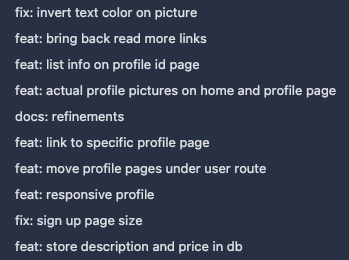
\includegraphics[width=8cm]{images/commit-log}
    \caption{Chronocademy's commit log}
    \label{fig:figure23}
\end{figure}

As the reader can see, the commit log is very descriptive, showing every step taken during the development process.\ For example, one commit is about configuring the ``profile page'' to be mobile responsive, the next one, still linked to the same feature, is about setting that page route, and so on.\ By following this practice, reading the commit log tells a story of how the development process went.\ Allowing developers to track changes and revert to a previous version if needed.\ This brought a lot of value to the project development phase.